 % The main file for CAMP reports
 % Don't put any content in here. 
 % Don't even include content files by using \input or \inlcude. 
 % Put your content to TEXT.TEX or include it there using \input.
 % Uses:
 %		SETTINGS.TEX		contains the settings for this document
 %		COMMANDS.TEX		contains commands which can be used while writing
 %		INFO.TEX			contains the author, title and so on for the cover
 %		COVER.TEX			formats the front cover of the document
 %		ABSTRACT.TEX		contains the abstract to be included (if needed)
 %		TEXT.TEX			contains the actual content of the document
 %		BIB.BIB				containt the BibTeX entries for the document
 


%% Draft document mode (with todos, no pictures just bounding box)
%\documentclass[draft,11pt,a4paper,bibtotoc,idxtotoc,headsepline,footsepline,footexclude,DIV13,oneside]{scrbook}
%% Final document mode (no todos, with pictures)
%\documentclass[final,11pt,a4paper,bibtotoc,idxtotoc,headsepline,footsepline,footexclude,DIV13,oneside]{scrbook}
%% Intermediate document mode (todos and pictures)
\documentclass[11pt,a4paper,bibtotoc,idxtotoc,headsepline,footsepline,footexclude,DIV13,oneside]{scrbook}
\usepackage{listings}
\lstset{basicstyle=\ttfamily,
  showstringspaces=false,
  commentstyle=\color{red},
  keywordstyle=\color{blue}
}
\usepackage[document]{ragged2e}
%\usepackage{epstopdf}
% KOMA-Optionen:
%  bibtotoc: include bibliography in table of contents
%  idxtotoc: include index in table of contents
%  headsepline: use horizontalline under heading
%  BCOR: binding correcion (Bindungskorrektur) (e.g.: BCOR5mm)
%  DIV: Number of sheet sections (used for layout) (e.g.: DIV12) 



% include title and author information for the cover
% Set here the title, authors and other stuff to be used for the cover
% This file is used by MAIN.TEX

% set title, authors and stuff for the cover
\def\doctype{BGCE Honours project report}
\def\title{CAD-integrated topology optimization}
\def\titleGer{CAD-integrierte Optimisierung von Topologie}
\def\author{S. Joshi, J.C. Medina, F. Menhorn, S. Reiz, B. Rüth, E. Wannerberg, A. Yurova}
\def\date{\today}

% text to appear in the footer
\def\footertext{}

% include settings
% Included by MAIN.TEX
% Defines the settings for the CAMP report document

\renewcommand{\sectfont}{\normalfont \bfseries}        % Schriftart der Kopfzeile

% manipulate footer
\usepackage{scrpage2}
\pagestyle{scrheadings}
\ifoot[\footertext]{\footertext} % \footertext set in INFO.TEX
%\setkomafont{pagehead}{\normalfont\rmfamily}
\setkomafont{pagenumber}{\normalfont\rmfamily}

%% allow sophisticated control structures
\usepackage{ifthen}

% use Palatino as default font
\usepackage{palatino}

% enable special PostScript fonts
\usepackage{pifont}

% make thumbnails
\usepackage{thumbpdf}

%to use the subfigures
\usepackage{subfigure}


\usepackage{colortbl}


%% show program code\ldots
%\usepackage{verbatim}
%\usepackage{program}

%% enable TUM symbols on title page
\usepackage{styles/tumlogo}


\usepackage{multirow}

%% use colors
\usepackage{color}

%% make fancy math
\usepackage{amsmath}
\usepackage{amsfonts}
\usepackage{amssymb}
\usepackage{textcomp}
\usepackage{yhmath} % fr die adots 
%% mark text as preliminary
%\usepackage[draft,german,scrtime]{prelim2e}

\usepackage{url}

%% create an index
\usepackage{makeidx}

% for the program environment
\usepackage{float}

%% load german babel package for german abstract
%\usepackage[german,american]{babel}
\usepackage[german,english]{babel}
\selectlanguage{english}

% use german characters as well
\usepackage[latin1]{inputenc}       % allow Latin1 characters

% use initals dropped caps - doesn't work with PDF
%\usepackage{dropping}
 %\usepackage[dvips]{dropping}

\usepackage{styles/shortoverview}
%----------------------------------------------------
%      Graphics and Hyperlinks
%----------------------------------------------------

%% check for pdfTeX
\ifx\pdftexversion\undefined
 %% use PostScript graphics
 \usepackage[dvips]{graphicx}

 \DeclareGraphicsExtensions{.eps,.epsi}
 \graphicspath{{figures/}{figures/review}{Pictures/}} 
 %% allow rotations
 \usepackage{rotating}
 %% mark pages as draft copies
 %\usepackage[english,all,light]{draftcopy}
 %% use hypertex version of hyperref
 \usepackage[hypertex,hyperindex=false,colorlinks=false]{hyperref}
\else %% reduce output size \pdfcompresslevel=9
 %% declare pdfinfo
 %\pdfinfo { 
 %  /Title (my title) 
 %  /Creator (pdfLaTeX) 
 %  /Author (my name) 
 %  /Subject (my subject	) 
 %  /Keywords (my keywords)
 %}
 %% use pdf or jpg graphics
 \usepackage[pdftex]{graphicx}
 \DeclareGraphicsExtensions{.jpg,.JPG,.png,.pdf,.eps}
 \graphicspath{{figures/}{Pictures/}} 
 
 %% Load float package, for enabling floating extensions
 \usepackage{float}
 
% \usepackage{mdframed}
 
 %% allow rotations
 \usepackage{rotating}
 %% use pdftex version of hyperref
 \usepackage[pdftex,pdfauthor={Joshi, Saumitra; Medina, Juan Carlos; Menhorn, Friedrich; Reiz, Severin; R{\"u}th, Benjamin; Wannerberg, Erik; Yurova, Anna},%
            pdftitle={CAD-integrated Topology Optimization},%
%            pdfsubject={The Subject},
            pdfkeywords={Topology Optimization, CAD description generation, CAD-integrated topology optimization},%
            colorlinks=true,linkcolor=black,citecolor=red,%
 anchorcolor=red,urlcolor=blue,bookmarks=true,%
 bookmarksopen=true,bookmarksopenlevel=0,plainpages=false%
 bookmarksnumbered=true,hyperindex=false,pdfstartview=%
 ]{hyperref}
%
%\usepackage[pdftex,colorlinks=false,linkcolor=red,citecolor=red,%
% anchorcolor=red,urlcolor=red,bookmarks=true,%
% bookmarksopen=true,bookmarksopenlevel=0,plainpages=false%
% bookmarksnumbered=true,hyperindex=false,pdfstartview=%
% ]{hyperref}
\fi
\usepackage{epstopdf}
\epstopdfsetup{update} % only regenerate pdf files when eps file is newer

\usepackage{listings} %source code formatter

% package for notes
\usepackage{todonotes}

%% Fancy chapters
%\usepackage[Lenny]{fncychap}
%\usepackage[Glenn]{fncychap}
%\usepackage[Bjarne]{fncychap}

%\usepackage[avantgarde]{quotchap}

% set the bibliography style
%\bibliographystyle{styles/bauermaNum}
%\bibliographystyle{alpha}
\bibliographystyle{unsrt}

% include commands
% Commands to be used within the TUM report document
% Included by MAIN.TEX
% Please include your own cool commands here. 
% Be only sure to comment it sufficiently so others can use it.

%-------------------------------------------------------------
%                      Own Commands
%-------------------------------------------------------------


%-------------------------------------------------------------
% math stuff -------------------------------------------------

% nice R, N, C
\newcommand{\nat}{\mathbb{N}}
\newcommand{\real}{\mathbb{R}}
\newcommand{\compl}{\mathbb{C}}


\newcommand{\dx}{\text{dx}}
\newcommand{\dt}{\text{dt}}

% norm
\newcommand{\norm}[1]{\left\| #1 \right\|}
\newcommand{\Ltwonorm}[1]{\norm{#1}_{L_2}}

% un demi
\newcommand{\half}{\frac{1}{2}}

% parantheses
\newcommand{\parenth}[1]{ \left( #1 \right) }
\newcommand{\bracket}[1]{ \left[ #1 \right] }
\newcommand{\accolade}[1]{ \left\{ #1 \right\} }
%\newcommand{\angle}[1]{ \left\langle  #1 \right\rangle }

% partial derivative: %#1 function, #2 which variable
% simple / single line version
\newcommand{\pardevS}[2]{ \delta_{#1} f(#2) }
% fraction version
\newcommand{\pardevF}[2]{ \frac{\partial #1}{\partial #2} }

% render vectors: 3 and 4 dimensional
\newcommand{\veciii}[3]{\left[ \begin{array}[h]{c} #1 \\ #2 \\ #3	\end{array} \right]}
\newcommand{\veciv}[4]{\left[ \begin{array}[h]{c} #1 \\ #2 \\ #3 \\ #4	\end{array} \right]}

% render matrices: 3  dimensional (arguments in row first order)
\newcommand{\matiii}[9]{\left[ \begin{array}[h]{ccc} #1 & #2 & #3 \\ #4 & #5 & #6 \\ #7 & #8 & #9	\end{array} \right]}
%DOESN'T WORK,DON'T KNOW WHY \newcommand{\mativ}[16]{\left[ \begin{array}[h]{cccc} #1 & #2 & #3 & #4 \\ #5 & #6 & #7 & #8 \\ #9 & #10 & #11 & #12 \\ #13 & #14 & #15 & #16 \end{array} \right]}


%-------------------------------------------------------------
%-------------------------------------------------------------


%-------------------------------------------------------------
% some abreviations ------------------------------------------
\newcommand{\Reg}{$^{\textregistered}$}
\newcommand{\reg}{$^{\textregistered}$ }
\newcommand{\Tm}{\texttrademark}
\newcommand{\tm}{\texttrademark~}
\newcommand {\bsl} {$\backslash$}

%-------------------------------------------------------------
%-------------------------------------------------------------


%-------------------------------------------------------------
% formating --------------------------------------------------

% Theorem & Co environments and counters
\newtheorem{theorem}{Theorem}[chapter]
\newtheorem{lemma}[theorem]{Lemma}
\newtheorem{corollary}[theorem]{Corollary}
\newtheorem{remark}[theorem]{Remark}
\newtheorem{definition}[theorem]{Definition}
\newtheorem{equat}[theorem]{Equation}
\newtheorem{example}[theorem]{Example}
\newtheorem{algorithm}[theorem]{Algorithm}

% inserting figures
\newcommand{\insertfigure}[4]{ % Filename, Caption, Label, Width percent of textwidth
	\begin{figure}[htbp]
		\begin{center}
			\includegraphics[width=#4\textwidth]{#1}
		\end{center}
		\vspace{-0.4cm}
		\caption{#2}
		\label{#3}
	\end{figure}
}




% referecing figures

\newcommand{\refFigure}[1]{ %label
	figure \ref{#1}
}
\newcommand{\refChapter}[1]{ %label
	chapter \ref{#1}
}

\newcommand{\refSection}[1]{ %label
	section \ref{#1}
}

\newcommand{\refParagraph}[1]{ %label
	paragraph \ref{#1}
}

\newcommand{\refEquation}[1]{ %label
	equation \ref{#1}
}

\newcommand{\refTable}[1]{ %label
	table \ref{#1}
}




\newcommand{\rigidTransform}[2]
{
	${}^{#2}\!\mathbf{H}_{#1}$
}

%code, in typewriter
\newcommand{\code}[1]
 {\texttt{#1}}

% comment that appears on the border - very practical !!!
\newcommand{\comment}[1]{\marginpar{\raggedright \noindent \footnotesize {\sl #1} }}

% page clearing
\newcommand{\clearemptydoublepage}{%
  \ifthenelse{\boolean{@twoside}}{\newpage{\pagestyle{empty}\cleardoublepage}}%
  {\clearpage}}


%-------------------------------------------------------------
%-------------------------------------------------------------


\newcommand{\etAl}{\emph{et al.}\mbox{ }}

% include acronyms and glossary
\acsetup{first-long-format=\itshape}

% class `abbrev': abbreviations:
\DeclareAcronym{DC}{
  short = DC ,
  long  = Dual Contouring ,
  class = abbrev
}
\DeclareAcronym{QEF}{
  short = QEF,
  long  = quadratic error function,
  class = abbrev
}
\DeclareAcronym{MC}{
  short = MC ,
  long  = Marching Cubes ,
  class = abbrev
}
\DeclareAcronym{DualMC}{
  short = DualMC ,
  long  = Dual Marching Cubes ,
  class = abbrev
}
\DeclareAcronym{DualMT}{
  short = DualMT ,
  long  = Dual Marching Tetrahedra ,
  class = abbrev
}
\DeclareAcronym{NURBS}{
  short = NURBS ,
  long  = Non-uniform Rational B-spline ,
  class = abbrev
}
\DeclareAcronym{Bspline}{
  short = B-spline ,
  long  = basis spline ,
  class = abbrev
}
\DeclareAcronym{CADTopOpt}{
  short = CADTopOpt,
  long = CAD-integrated Topology Optimization,
  class = abbrev
}
\DeclareAcronym{CAD}{
  short = CAD,
  long = Computer Aided Design,
  class = abbrev
}
\DeclareAcronym{CSG}{
  short = CSG,
  long = constructive solid geometry,
  class = abbrev
}
\DeclareAcronym{BREP}{
  short = BREP,
  long = boundary representation,
  class = abbrev
}
\DeclareAcronym{STL}{
  short = STL,
  long = stereo lithography,
  class = abbrev
}
\DeclareAcronym{STEP}{
  short = STEP,
  long = standard for the exchange of product model data,
  class = abbrev
}
\DeclareAcronym{IGES}{
  short = IGES,
  long = Initial Graphics Exchange Specification,
  class = abbrev
}
% class `nomencl': nomenclature
\DeclareAcronym{quad}{
  short = quad ,
  long  = quadrilateral face ,
  class = nomencl
}
\DeclareAcronym{tri}{
  short = triangle,
  long = triangular face,
  class = nomencl
}
\DeclareAcronym{patch}{
  short = patch,
  short-plural = es, 
  long  = a patch of rectangular topology,
  long-plural-form = patches of rectangular topology,
  class = nomencl
}
\DeclareAcronym{voxel}{
  short = voxel,
  long = a cube with uniform edge length and a datavalue on each corner of the cube,
  class = nomencl
}
\DeclareAcronym{FirstOrderHermiteData}{
  short = first order Hermite data,
  long = first derivative (gradient respectively) and value of a function at a certain point,
  class = nomencl
}
\DeclareAcronym{SignChangingEdge}{
  short = sign changing edge,
  long = an edge which has vertex values both above and below the isovalue,
  class = nomencl
}

\makeglossary

\begin{document}

	\frontmatter
	
	% The titlepage for the CAMP report document.
% Included by MAIN.TEX


%--------------------------------------------------
% The title page
%--------------------------------------------------

% correct BCOR - undo at the end !!!
\def\bcorcor{0.15cm}
\addtolength{\hoffset}{\bcorcor}

\thispagestyle{empty}

 \vspace{10mm}
\begin{center}
	       %\oTUM{4cm}
	       
\includegraphics[width=4cm]{styles/tum_logo.png}
	   
	   \vspace{5mm}     
	   \huge Bavarian Graduate School of Computational Engineering \\Honours project\\ 
	   \vspace{0.5cm}
	 \large Technische Universit{\"a}t M{\"u}nchen\\
        
	\end{center}
		

\vspace{10mm}
\begin{center}

   {\Large \doctype}

  \vspace{10mm}
  
  {\LARGE \title}\\
  
  
  \vspace{10mm}
  
  
  %{\LARGE  \titleGer}\\
  
  
  %\vspace{10mm}

    %\hfill
    \begin{tabular}{ll}
	   \Large Authors:     & \Large \author \\[2mm]
%	   \Large $\mathrm{1^{st}}$ examiner:    & \Large Prof. Dr. However Wasit \\[2mm]				
%	   \Large $\mathrm{2^{nd}}$ examiner:    & \Large Prof. Dr. However Wasit \\[2mm]
	   \Large Advisors:    & \Large Arash, Dirk an Utz... \\[2mm]
%	   \Large Thesis handed in on:       & \Large August 15, 2006
	 \end{tabular}
	 
	 \vspace{5mm}
	 
	 \begin{figure}[h!]
  \centering
   
\includegraphics[width=\textwidth]{styles/sccs_os2.pdf}
  \end{figure}
   

\end{center}

% undo BCOR correction
\addtolength{\hoffset}{\bcorcor}
	
	\clearemptydoublepage
\phantomsection
\addcontentsline{toc}{chapter}{Preface}	


\vspace*{3cm}

\begin{flushleft}
{\Large \bf Preface}
\end{flushleft}

\vspace{1cm}
The Bavarian Graduate School of Computational Engineering (BGCE) honours project at the Computational Science and Engineering (CSE) Institute of Technische Universitaet Muenchen (TUM) is a 10-month project where students conduct research on cutting-edge topics in the field of Computational Engineering, in cooperation with a partner in industry or academia. The 2015-16 project is titled \emph{CAD-Integrated Topology Optimization} and is initiated and supervised in a cooperation between TUM and Siemens AG in Munich.


\newpage

	
	%\clearemptydoublepage


\thispagestyle{empty}
\selectlanguage{english}
	\vspace*{0.8\textheight}
	\noindent
	I hereby declare that this thesis is entirely the result of my own work except where otherwise indicated. I have only used the resources given in the list of references.
	
	\vspace{15mm}
	\noindent
	\today \hspace{5cm} \author
\selectlanguage{english}
\newpage
	
	%\clearemptydoublepage
\phantomsection
\addcontentsline{toc}{chapter}{Acknowledgements}	


%\chapter*{Acknowledgements}

\vspace*{2cm}

\begin{center}
{\Large \bf Acknowledgments}
\end{center}

\vspace{1cm}

This Honour's project is carried out under the supervision of Dr. Dirk Hartmann, , Dr. Utz Wever  from the side of the customer (Siemens AG) and Arash Bakhtiari (TUM). We would like to thank Bavarian Graduate School of Computational Engineering for providing us an opportunity to participate in a project closely related to the industry in a highly relevant and challenging topic.
	
	%% Abstract for the TUM report document
% Included by MAIN.TEX


\clearemptydoublepage
\phantomsection
\addcontentsline{toc}{chapter}{Abstract}	





\vspace*{2cm}
\begin{center}
{\Large \bf Abstract}
\end{center}
\vspace{1cm}

Topology optimization is becoming an increasingly important tool in computer aided design (CAD). Several topology optimization open-source tools already exist; however,  it can still be cumbersome to incorporate these tools efficiently in the design process. The main challenge lies in converting mesh-based topology optimized solutions to a smooth geometry representation. We address this issue with a two-stage Dual Contouring surface reconstruction scheme for coarse parametrization patches and fine vertices. A B-Spline surface is fitted by a least-square approach using control points described by the Peters' scheme. This ensures geometrically continuous surfaces. In conclusion, a fully CAD-integrated topology optimization tool-chain is provided.

	\listoftodos
	\tableofcontents
  	%outline and overview

	\mainmatter
	
	\chapter{Introduction}
	\label{intro}
	In this document we provide a complete guide on how to install and use CADTOPCAD tool on Linux.

	\chapter{ToPy}
	\label{Topy}
	In our tool we use ToPy (\href{https://github.com/williamhunter/topy}{https://github.com/williamhunter/topy}) for topology optimization. 
	\section{Prerequisites}
	\label{ToPy:sec1}
	In order to install ToPy, make sure that the following software is installed on your computer:
	\begin{itemize}
	\item Python (version $>$ 2.7)
	\item NumPy (Usually provided by Python distribution)
	\item PyVTK tool (\href{https://pypi.python.org/pypi/PyVTK}{https://pypi.python.org/pypi/PyVTK}) 
	\item Pysparse library(\href{http://pysparse.sourceforge.net/}{http://pysparse.sourceforge.net/})
	\end{itemize}
	Here are some recommendation for the installation of the above mentioned tools/libraries.
	
	To install PyVTK tool, please run the following commands in your terminal:
\begin{lstlisting}[language=bash]
sudo apt-get install python-pip
sudo pip install pyvtk
\end{lstlisting}	
	%\end{flushleft}
	
	
	The installation of the Pysparse library is a little bit more cumbersome, since the pip-installation (like in the previous case) fails most of the times. So, here we provide an alternative way of installing Pysparse from the \textit{.git} repository.
	
	To install Pysparse, make sure that \textit{git} (\href{https://git-scm.com/}{url}) is installed on your computer and then run the following commands in your terminal:
\begin{lstlisting}[language=bash]
git clone git:://pysparse.git.sourceforge.net/gitroot/pysparse/pysparse/
\item cd pysparse
\item sudo python setup.py install	
\end{lstlisting}	
	
	Furthermore, for CADTOPCAD it is necessary to have an output in the \textit{ascii} format. By default the output \textit{.vtk} files from ToPy are binary, so we need to change them to \textit{ascii}. In order to do that, please perform the following actions:
	\begin{itemize}
 		\item Open the ToPy source file \texttt{core/visualization.py}
 		\item Go to the method \texttt{{\_}write{\_}legace{\_}vtu(x, fname)} (line 160)
 		\item Change in line 194 \texttt{binary} to \texttt{ascii} (see pic. \ref{fig:ToPy_CodeChange})
	\end{itemize} 
	\begin{figure}
	\centering
	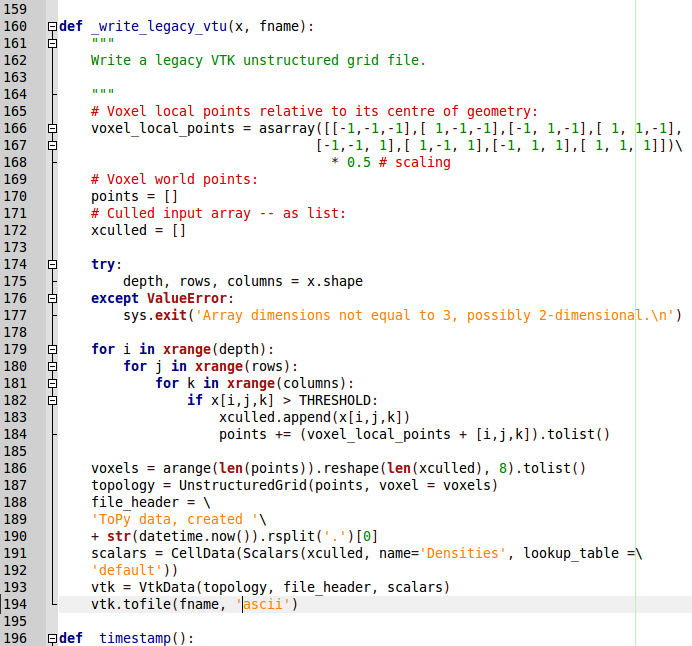
\includegraphics[scale=0.5]{img/ToPy_CodeChange.png}
	\caption{Changing of the output type of ToPy to ascii}
	\label{fig:ToPy_CodeChange}
	\end{figure}
	

	\section{Install ToPy}
	If all the tools specified in the section \ref{ToPy:sec1} are installed, we can now proceed to the installation of ToPy itself. For that download ToPy from \href{https://github.com/williamhunter/topy}{https://github.com/williamhunter/topy} \todo{Did we clone it from git or downloaded it?} and run the following command from the root directory of ToPy:
\begin{lstlisting}[language=bash]
sudo python setup.py install
\end{lstlisting}	
	\begin{figure}
	\centering
	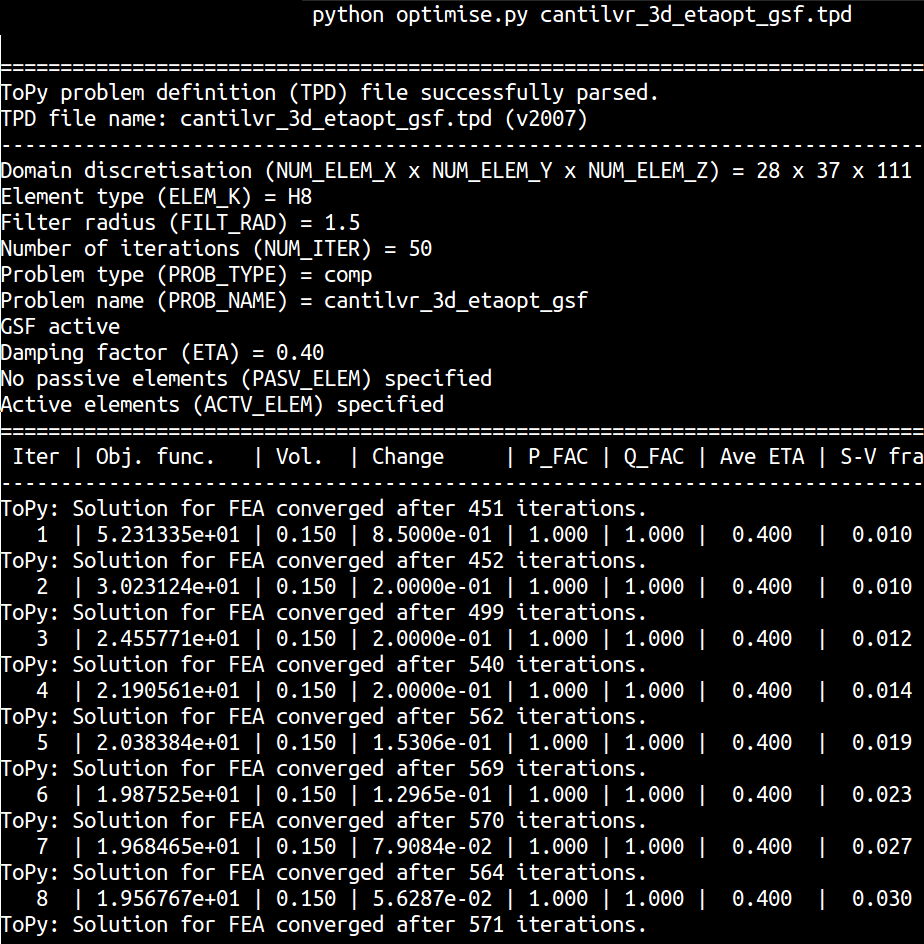
\includegraphics[scale=0.2]{img/ToPy_ExampleRun.png}
	\caption{ToPy test}
	\label{fig:ToPy_test}
	\end{figure}


	\section{Test ToPy}
	In order to test whether the installation of ToPy was completed successfully it is possible to run some test cases provided in \textit{examples} folder. For that, do the following:
	\begin{itemize}
	\item Enter one of the folders in examples (e.g. examples/cantilever)
	\item Execute a ToPy test run by running the following command in your terminal:
\begin{lstlisting}[language=bash]
python optimize.py <example.tpd-file>
\end{lstlisting}	
	\end{itemize}
	
The output should look as showed on a picture \ref{fig:ToPy_test}.


\chapter{OpenCascade}
\label{OpenCascade}
OpenCascade (\href{http://www.opencascade.com/}{http://www.opencascade.com/}) is a... \todo{maybe add a short description}
\section{Install OpenCascade}
For technical reasons, we do not use OpenCascade from the official webpage, but from the \textit{.git} repository. 
\begin{figure}
\centering
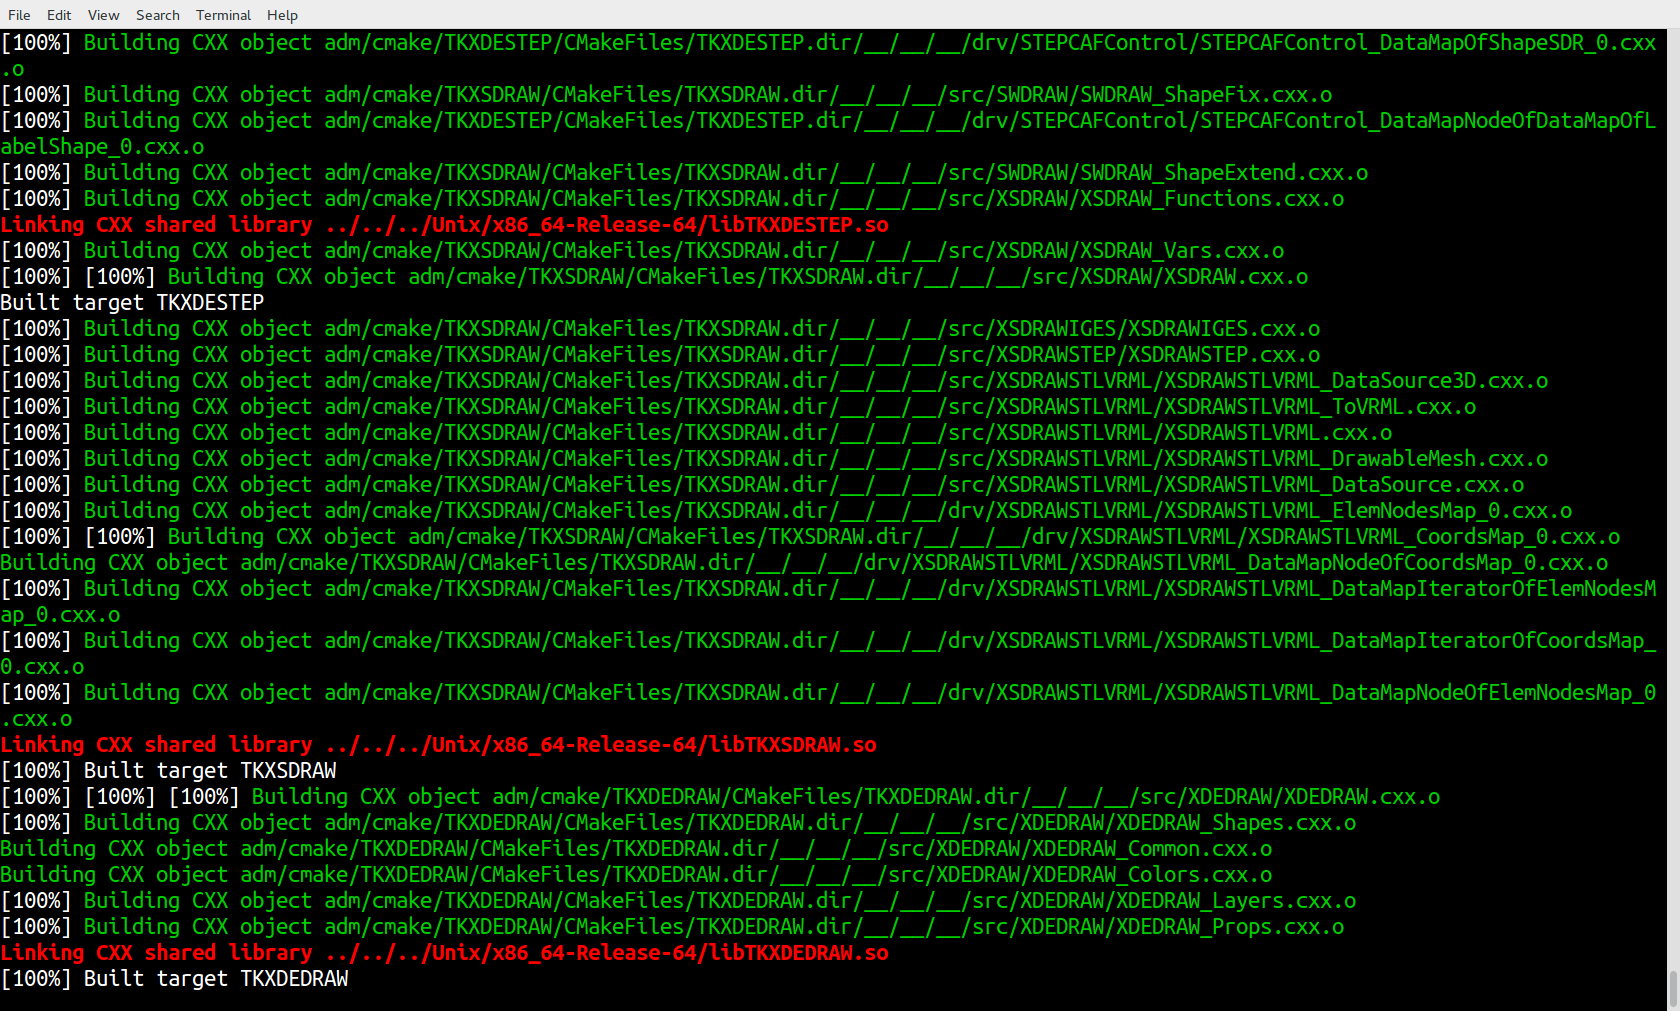
\includegraphics[scale=0.2]{img/OC_Build5.png}
\caption{Building OpenCascade}
\label{fig:OC_build}
\end{figure}
\begin{figure}
\centering
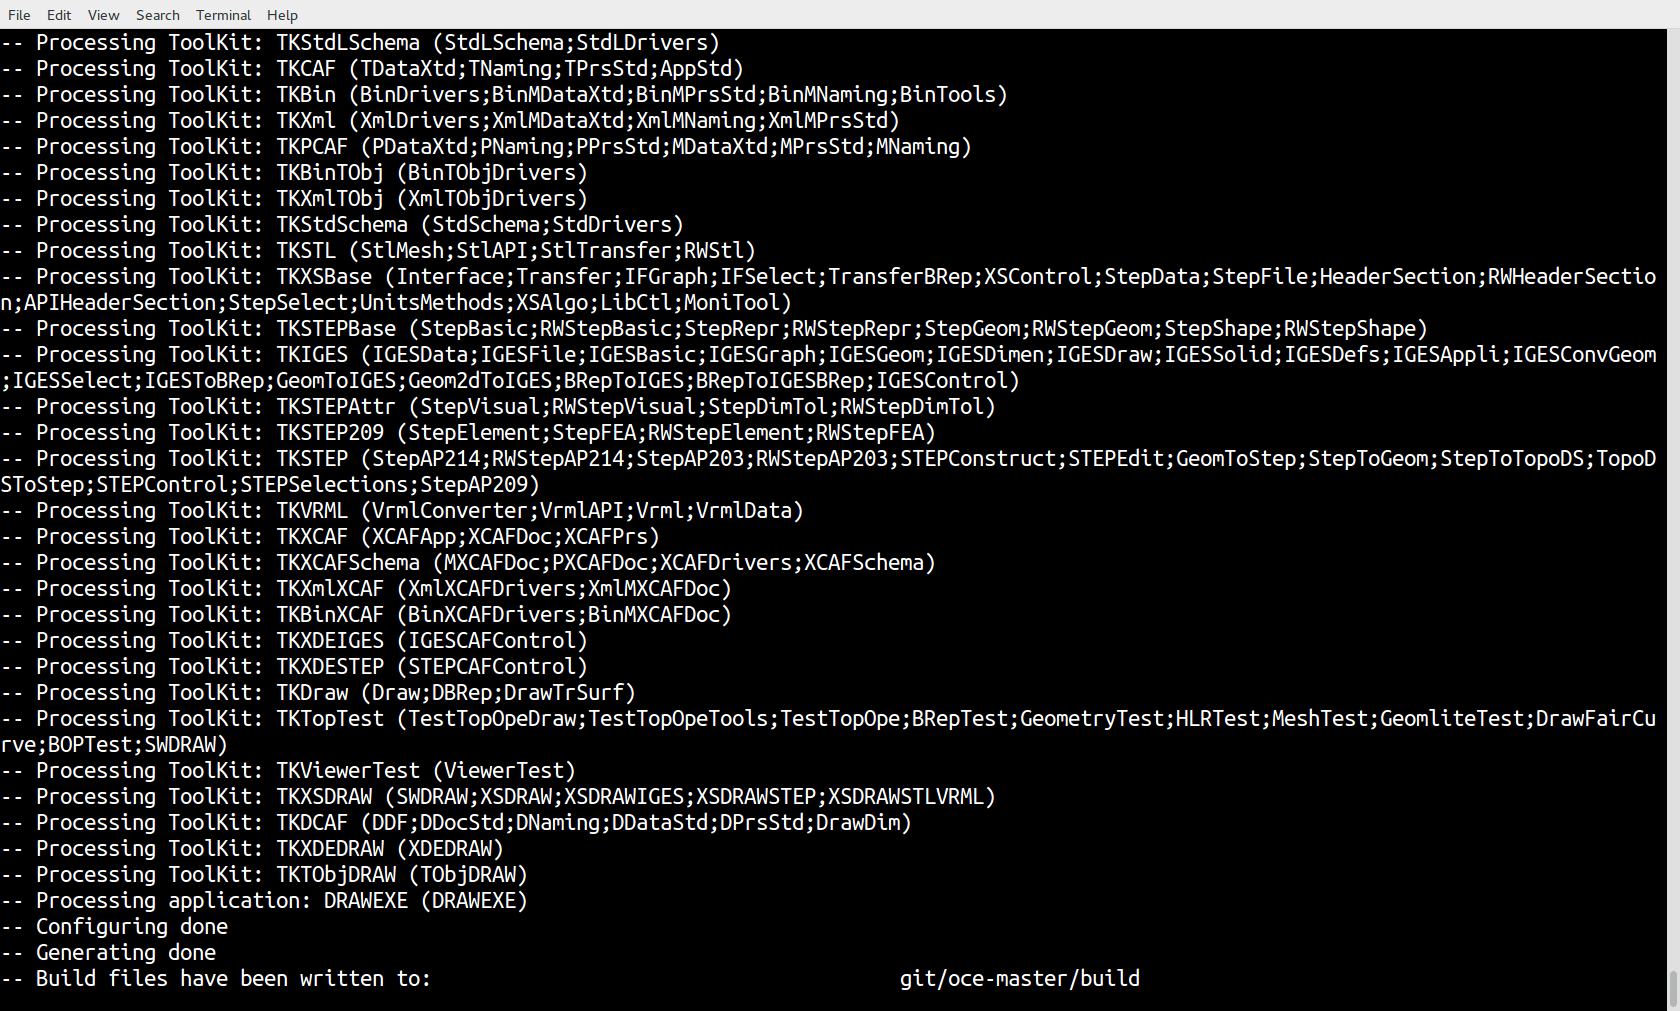
\includegraphics[scale=0.3]{img/OC_CMake2.png}
\caption{OpenCascade installation: cmake}
\label{fig:OC_cmake}
\end{figure}
To install OpenCascade this way, make sure that textit{git} (\href{https://git-scm.com/}{url}) is installed on your computer and then run the following commands in your terminal:
\begin{itemize}
\item \begin{lstlisting}[language=bash]
git clone git://github.com/tpaviot/oce.git
cd oce
mkdir build
cd build
\end{lstlisting}
	
\item 
\begin{lstlisting}[language=bash]
cmake .. 
\end{lstlisting}	
Sample output: see Pic. \ref{fig:OC_build}
\item 
\begin{lstlisting}[language=bash]
make .. 
\end{lstlisting}	
Sample output: see Pic. \ref{fig:OC_cmake}
\item 
\begin{lstlisting}[language=bash]
sudo make install .. 
\end{lstlisting}	
Sample output: see Pic. \ref{fig:OC_install}
\end{itemize}

\begin{figure}
\centering
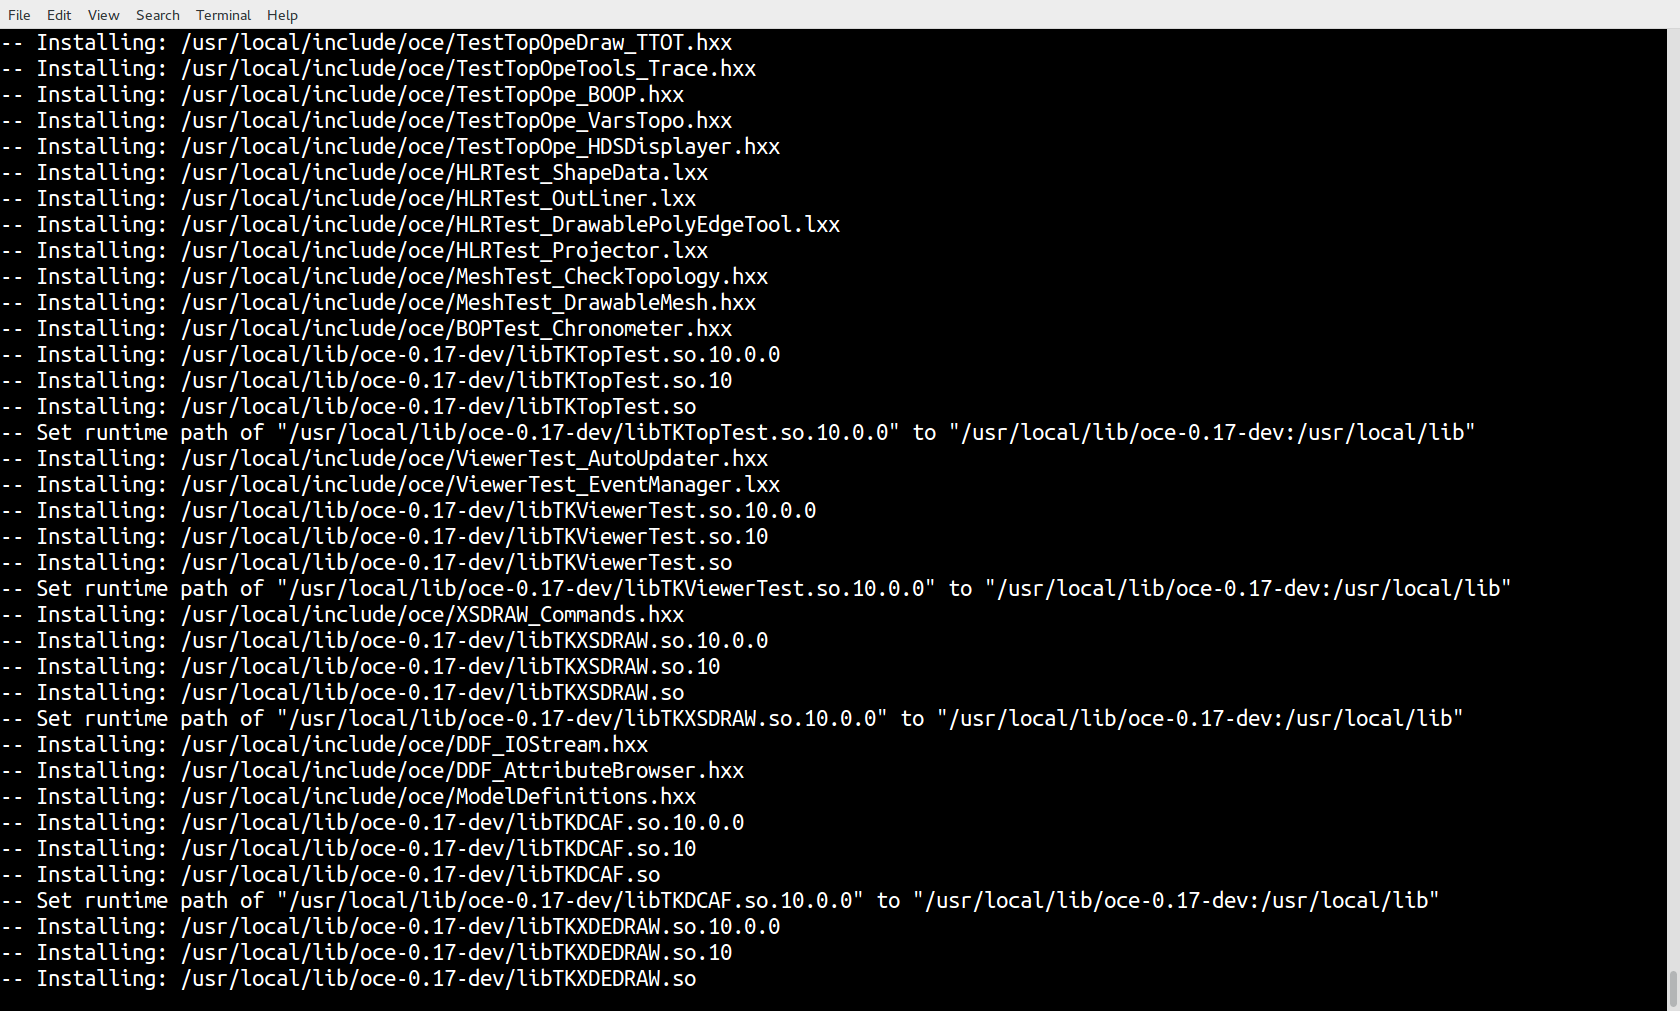
\includegraphics[scale=0.3]{img/OC_Install2.png}
\caption{OpenCascade installation}
\label{fig:OC_install}
\end{figure}
	In the make step, one can use the \texttt{-jx} parameter, where $x$ is the number of processors, to build in parallel. That allows to speed up the installation process These steps are in accord with the installation guide on the git page itself. One can also use the CMake-GUI (see Pic. \ref{fig:CMake_GUI}) to change some of the build configuration if need be (e.g. include OpenMP support).
	
\begin{figure}
\centering
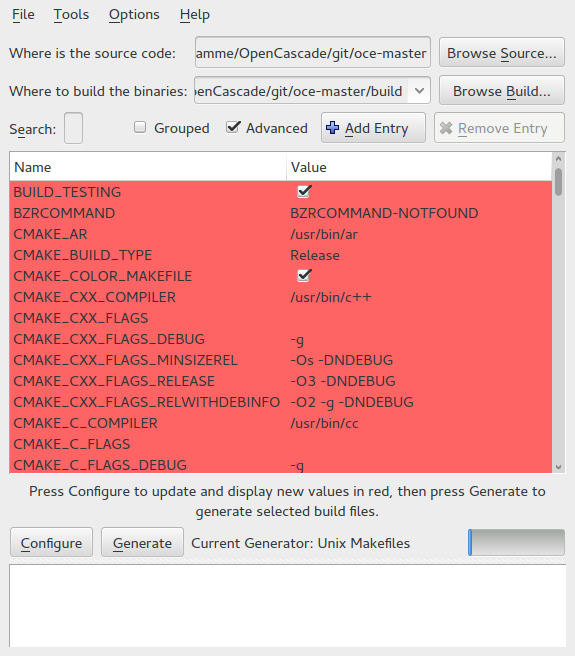
\includegraphics[scale=0.5]{img/CMake_GUI.png}
\caption{CMake graphical interface}
\label{fig:CMake_GUI}
\end{figure}
\section{Test OpenCascade}
\begin{figure}
\centering
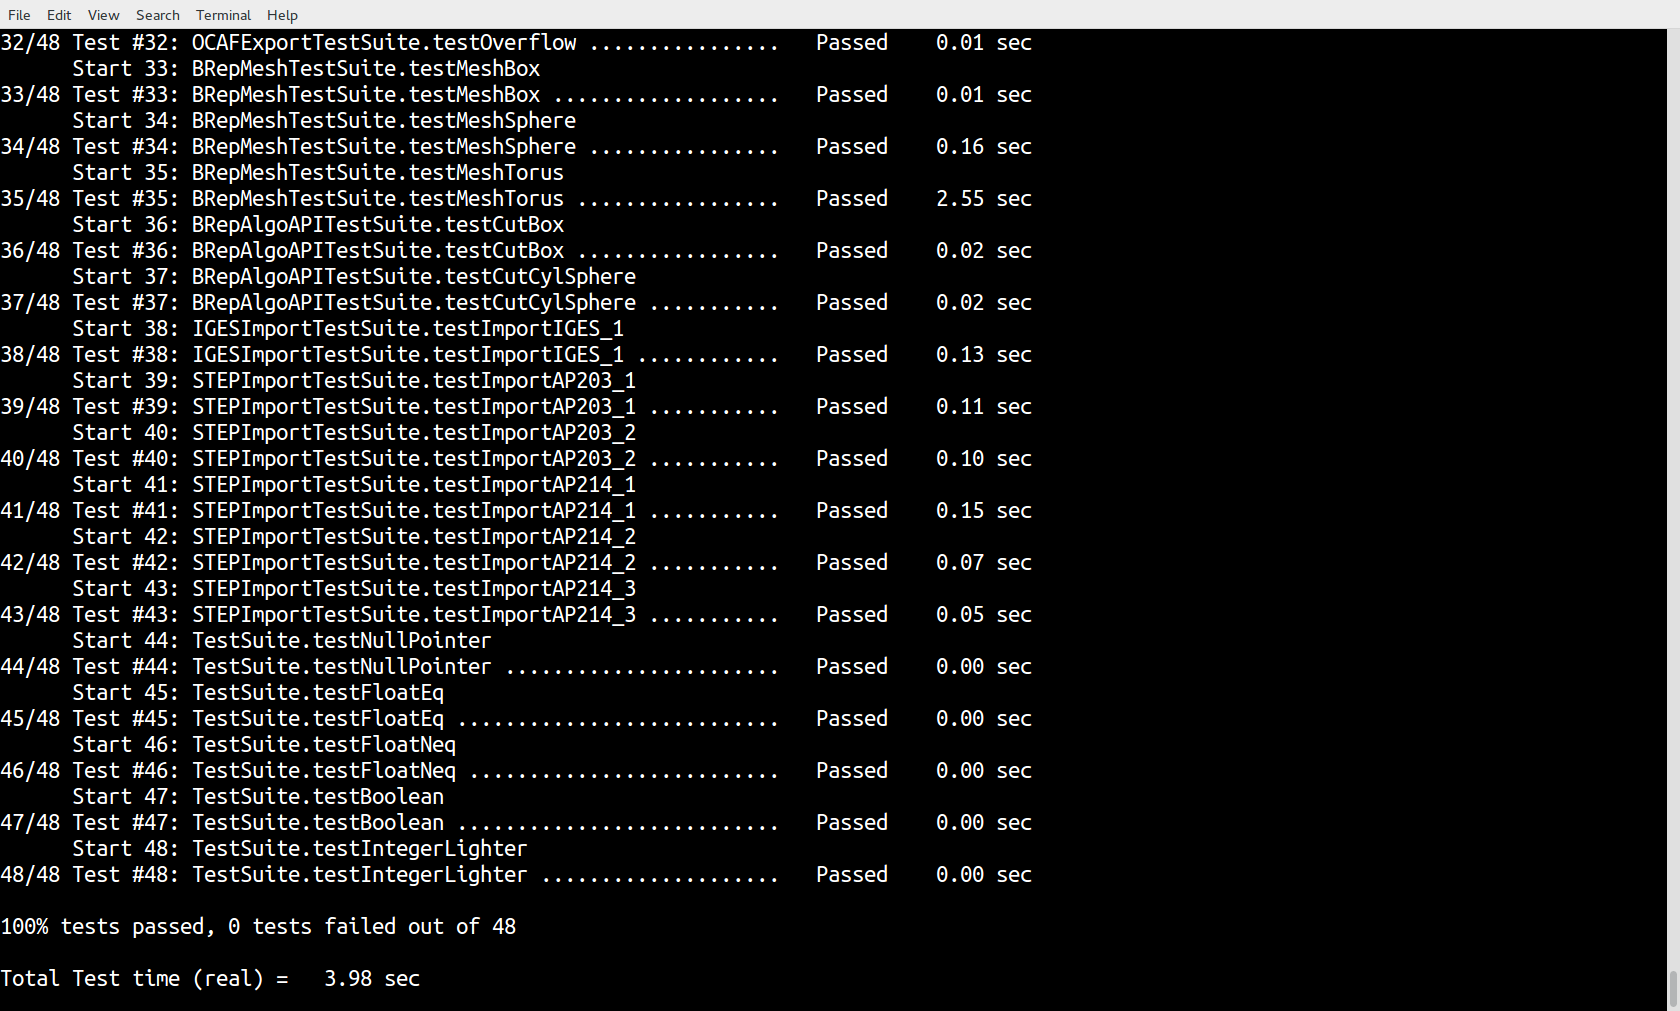
\includegraphics[scale=0.2]{img/OC_Test2.png}
\caption{OpenCascade test}
\label{fig:OC_test}
\end{figure}
In order to test whether the installation of OpenCascade was completed successfully it is possible to run a test provided by OpenCascade. 

For that, run the following command from your terminal:
\begin{lstlisting}[language=bash]
make test
\end{lstlisting}
All performed tests should be successful (See Pic. \ref{fig:OC_test})


\chapter{CADTOPCAD}
\section{Prerequisites}
In order to install CADTOPCAD the following tools should be installed on your computer:
\begin{itemize}
	\item Topy (see Sec. \ref{Topy})
	\item OpenCascade (see Sec. \ref{OpenCascade})
	\item (\href{http://cppunit.sourceforge.net/doc/cvs/cppunit_cookbook.html}{CPPUnit})
	\end{itemize}
In order to install CPPUnit run the following command from you terminal:
\begin{lstlisting}[language=bash]
sudo apt-get install lib-cppunitdev
\end{lstlisting}

  	\clearemptydoublepage
	
 
\end{document}

